\documentclass[11pt,a4paper]{article}

\usepackage[utf8]{inputenc}
\usepackage[T1]{fontenc}
\usepackage{lmodern}
\usepackage[margin=0.72in]{geometry}
\usepackage[table]{xcolor}
\usepackage{array}
\usepackage{tabularx}
\usepackage{booktabs}
\usepackage{enumitem}
\usepackage{titlesec}
\usepackage{fancyhdr}
\usepackage{lastpage}
\usepackage{hyperref}
\usepackage{tikz}

\definecolor{TextInk}{HTML}{233142}
\definecolor{HeadingBlue}{HTML}{1D3557}
\definecolor{AccentTeal}{HTML}{2A7F92}
\definecolor{AccentGold}{HTML}{C58B4E}
\definecolor{RuleGray}{HTML}{D6E0E5}
\definecolor{TableStripe}{HTML}{F3F8FA}
\definecolor{SoftTint}{HTML}{F7F4EE}
\definecolor{SoftBlue}{HTML}{EEF6F8}
\definecolor{SoftGreen}{HTML}{EEF7F0}
\definecolor{SoftRed}{HTML}{FBF0EF}

\hypersetup{
  colorlinks=true,
  linkcolor=HeadingBlue,
  urlcolor=AccentTeal,
  pdftitle={IB Geography SL Paper 1 Full Simulation - 2026-05-02},
  pdfauthor={IB Geography SL Preparation}
}

\color{TextInk}
\setlength{\parskip}{0.48em}
\setlength{\parindent}{0pt}
\setlength{\tabcolsep}{5pt}
\renewcommand{\arraystretch}{1.17}
\setlist[enumerate]{leftmargin=1.55em,itemsep=5pt,topsep=5pt}
\setlist[itemize]{leftmargin=1.35em,itemsep=3pt,topsep=4pt}

\newcolumntype{Y}{>{\raggedright\arraybackslash}X}
\newcolumntype{L}[1]{>{\raggedright\arraybackslash}p{#1}}
\newcolumntype{C}[1]{>{\centering\arraybackslash}p{#1}}

\titleformat{\section}
  {\normalfont\huge\sffamily\bfseries\color{HeadingBlue}}
  {}{0pt}{}
  [\vspace{0.12em}{\color{AccentGold}\titlerule[1pt]}]

\titleformat{\subsection}
  {\normalfont\Large\sffamily\bfseries\color{AccentTeal}}
  {}{0pt}{}

\titleformat{\subsubsection}
  {\normalfont\large\sffamily\bfseries\color{HeadingBlue}}
  {}{0pt}{}

\titlespacing*{\section}{0pt}{1.1em}{0.5em}
\titlespacing*{\subsection}{0pt}{0.85em}{0.25em}
\titlespacing*{\subsubsection}{0pt}{0.65em}{0.2em}

\pagestyle{fancy}
\setlength{\headheight}{14pt}
\fancyhf{}
\fancyhead[L]{\sffamily\color{AccentTeal}Sat 2026-05-02}
\fancyhead[R]{\sffamily\color{HeadingBlue}Paper 1 Simulation}
\fancyfoot[C]{\sffamily\color{HeadingBlue}\thepage\ of \pageref{LastPage}}
\renewcommand{\headrulewidth}{0.4pt}
\renewcommand{\footrulewidth}{0pt}

\newcommand{\term}[1]{\textcolor{HeadingBlue}{\textbf{#1}}}
\newcommand{\exam}[1]{\textcolor{AccentTeal}{\textbf{#1}}}
\newcommand{\markpts}[1]{\hfill\textbf{[#1]}}
\newcommand{\boxnote}[3]{%
\noindent\colorbox{#1}{%
  \begin{minipage}{0.965\textwidth}
  \sffamily
  \textbf{\textcolor{HeadingBlue}{#2}} #3
  \end{minipage}
}}

\begin{document}

\begin{center}
  {\sffamily\bfseries\color{HeadingBlue}\LARGE IB Geography SL}\\[0.2em]
  {\sffamily\bfseries\color{AccentTeal}\Large Paper 1 Full Simulation}\\[0.3em]
  {\sffamily\color{TextInk}Saturday 2026-05-02: Urban Environments + Food And Health}
\end{center}

\vspace{0.35em}

\boxnote{SoftRed}{Practice-paper notice.}{This is an IB-style practice paper
created for revision. It is not an official IB past paper or official IB mark
scheme. Use it only after putting notes away.}

\section{Instructions}

\begin{tabularx}{\textwidth}{L{0.25\textwidth}Y}
\toprule
\textbf{Total time} & \term{1 hour 30 minutes}. Spend \term{45 minutes} on
Urban environments and \term{45 minutes} on Food and health. \\
\textbf{Total marks} & \term{40 marks}. Each option is worth \term{20 marks}. \\
\textbf{Materials} & Question paper, answer booklet, timer, and pen. Do not use
notes during the simulation. \\
\textbf{Structure} & Answer every structured question. For each option, choose
\term{one} of the two 10-mark extended-answer prompts. \\
\textbf{Review} & Mark the paper immediately after if time allows. If not,
carry the marking guide and error log into the May 4 remediation block. \\
\bottomrule
\end{tabularx}

\subsection{Timing Checkpoints}

\rowcolors{2}{TableStripe}{white}
\begin{tabularx}{\textwidth}{L{0.18\textwidth}Y L{0.2\textwidth}}
\toprule
\textbf{Minute} & \textbf{Action} & \textbf{Marks done} \\
\midrule
0--2 & Read the Urban source and questions. & 0 \\
2--20 & Answer Urban structured questions 1--3. & 10 \\
20--45 & Choose and write one Urban 10-mark answer. & 20 \\
45--47 & Switch quickly to Food and health. & 20 \\
47--65 & Answer Food and health structured questions 1--3. & 30 \\
65--90 & Choose and write one Food and health 10-mark answer. & 40 \\
\bottomrule
\end{tabularx}
\rowcolors{2}{}{}

\newpage

\section{Option G: Urban Environments}

\subsection{Source A: Four Urban Zones In One Large City}

Source A shows selected characteristics of four zones in a large city. The
data are illustrative and are provided for interpretation practice.

\rowcolors{2}{TableStripe}{white}
\begin{tabularx}{\textwidth}{L{0.18\textwidth}C{0.15\textwidth}C{0.16\textwidth}C{0.14\textwidth}Y}
\toprule
\textbf{Zone} & \textbf{Population density} & \textbf{Average monthly rent index}
& \textbf{Green space} & \textbf{Main issue} \\
\midrule
Central business district & Medium at night; very high by day & 100 & 8\% &
Congestion, high land value, and limited space for housing \\
Inner-city regeneration zone & High & 82 & 14\% & Rising rents, reuse of
former industrial land, and possible displacement \\
Suburban residential zone & Medium to low & 58 & 34\% & Longer commuting,
car dependence, and land consumption \\
Peripheral informal settlement & Very high & 24 & 3\% & Insecure housing,
weak service access, and flood or pollution exposure \\
\bottomrule
\end{tabularx}
\rowcolors{2}{}{}

\subsubsection{Visual Source A}

The chart compares the four zones using a 0--100 index. Higher bars show a
higher value for the selected indicator.

\begin{center}
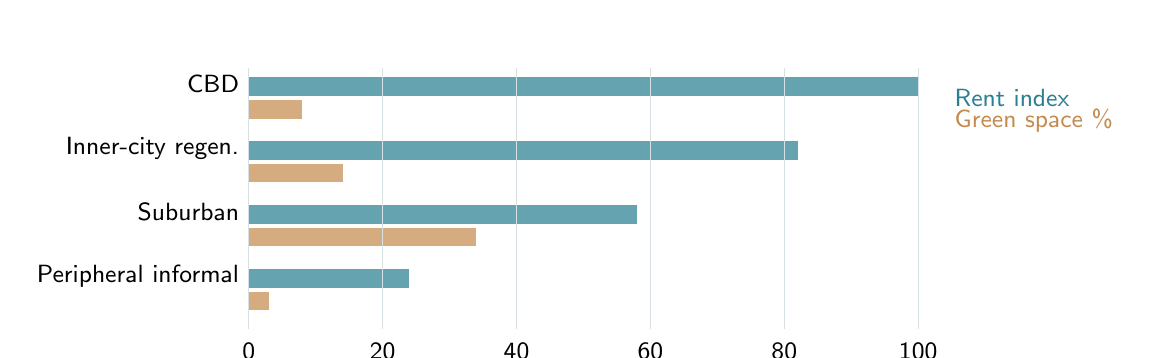
\begin{tikzpicture}[x=0.085cm,y=0.58cm, every node/.style={font=\sffamily\small}]
  \node[anchor=east] at (0,6.2) {CBD};
  \draw[fill=AccentTeal!72, draw=none] (0,5.95) rectangle (100,6.35);
  \draw[fill=AccentGold!72, draw=none] (0,5.45) rectangle (8,5.85);
  \node[anchor=east] at (0,4.8) {Inner-city regen.};
  \draw[fill=AccentTeal!72, draw=none] (0,4.55) rectangle (82,4.95);
  \draw[fill=AccentGold!72, draw=none] (0,4.05) rectangle (14,4.45);
  \node[anchor=east] at (0,3.4) {Suburban};
  \draw[fill=AccentTeal!72, draw=none] (0,3.15) rectangle (58,3.55);
  \draw[fill=AccentGold!72, draw=none] (0,2.65) rectangle (34,3.05);
  \node[anchor=east] at (0,2.0) {Peripheral informal};
  \draw[fill=AccentTeal!72, draw=none] (0,1.75) rectangle (24,2.15);
  \draw[fill=AccentGold!72, draw=none] (0,1.25) rectangle (3,1.65);
  \foreach \x in {0,20,40,60,80,100} {
    \draw[RuleGray] (\x,0.85) -- (\x,6.55);
    \node[anchor=north] at (\x,0.75) {\x};
  }
  \node[anchor=west, color=AccentTeal] at (104,5.9) {Rent index};
  \node[anchor=west, color=AccentGold] at (104,5.4) {Green space \%};
\end{tikzpicture}
\end{center}

\subsection{Questions}

Answer all parts. For Question 4, answer either \term{4(a)} or \term{4(b)}.

\begin{enumerate}
  \item \exam{State} two pieces of evidence from Source A that show uneven
  environmental quality between urban zones. \markpts{2}

  \item \exam{Describe} two contrasts between the inner-city regeneration zone
  and the peripheral informal settlement shown in Source A. \markpts{4}

  \item \exam{Explain} two reasons why rapid urban growth can create social or
  environmental stress. \markpts{4}

  \item Answer either 4(a) or 4(b). \markpts{10}
  \begin{enumerate}[label=\textbf{\alph*.},leftmargin=1.6em]
    \item Using one named city, \exam{examine} the success of strategies to
    manage urban social or environmental stress sustainably.

    \item Using one or more named examples, \exam{to what extent} can
    regeneration or gentrification solve problems caused by urban decline?
  \end{enumerate}
\end{enumerate}

\newpage

\section{Option F: Food And Health}

\subsection{Source B: Food And Health Indicators For Three Regions}

Source B shows illustrative indicators for three regions at different stages
of food-system and health-system change.

\rowcolors{2}{TableStripe}{white}
\begin{tabularx}{\textwidth}{L{0.27\textwidth}C{0.18\textwidth}C{0.18\textwidth}C{0.18\textwidth}}
\toprule
\textbf{Indicator} & \textbf{Region X} & \textbf{Region Y} & \textbf{Region Z} \\
\midrule
Dominant food-system issue & Limited access and weak storage & Transitioning
diets and uneven access & High processed-food consumption \\
Households reporting food insecurity & 38\% & 18\% & 7\% \\
Child undernutrition & 28\% & 11\% & 3\% \\
Adult obesity & 6\% & 19\% & 32\% \\
Access to safe water & 62\% & 84\% & 98\% \\
Most likely health concern & Water-borne and infectious disease risk & Mixed
communicable and diet-related disease burden & Diet-related non-communicable
disease risk \\
\bottomrule
\end{tabularx}
\rowcolors{2}{}{}

\subsubsection{Visual Source B}

The chart compares food insecurity, child undernutrition, and adult obesity.

\begin{center}
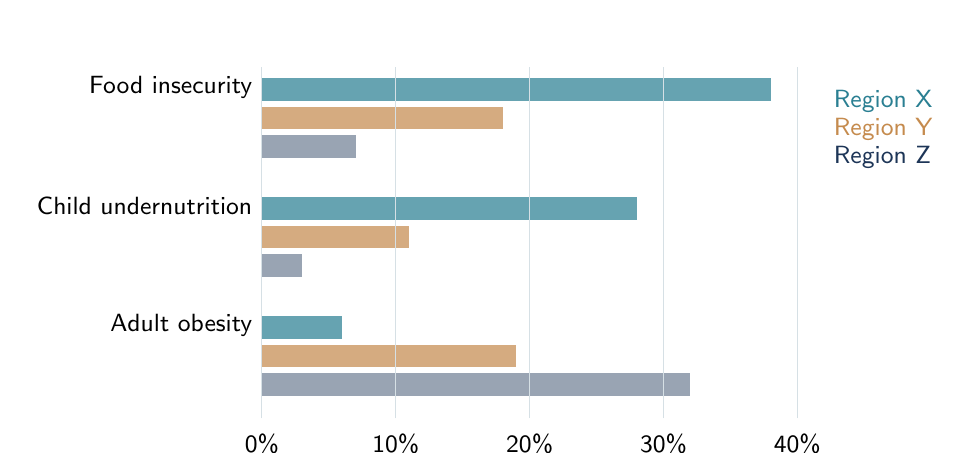
\begin{tikzpicture}[x=0.17cm,y=0.72cm, every node/.style={font=\sffamily\small}]
  \node[anchor=east] at (0,6.2) {Food insecurity};
  \draw[fill=AccentTeal!72, draw=none] (0,5.95) rectangle (38,6.35);
  \draw[fill=AccentGold!72, draw=none] (0,5.45) rectangle (18,5.85);
  \draw[fill=HeadingBlue!45, draw=none] (0,4.95) rectangle (7,5.35);
  \node[anchor=east] at (0,4.1) {Child undernutrition};
  \draw[fill=AccentTeal!72, draw=none] (0,3.85) rectangle (28,4.25);
  \draw[fill=AccentGold!72, draw=none] (0,3.35) rectangle (11,3.75);
  \draw[fill=HeadingBlue!45, draw=none] (0,2.85) rectangle (3,3.25);
  \node[anchor=east] at (0,2.0) {Adult obesity};
  \draw[fill=AccentTeal!72, draw=none] (0,1.75) rectangle (6,2.15);
  \draw[fill=AccentGold!72, draw=none] (0,1.25) rectangle (19,1.65);
  \draw[fill=HeadingBlue!45, draw=none] (0,0.75) rectangle (32,1.15);
  \foreach \x in {0,10,20,30,40} {
    \draw[RuleGray] (\x,0.35) -- (\x,6.55);
    \node[anchor=north] at (\x,0.25) {\x\%};
  }
  \node[anchor=west, color=AccentTeal] at (42,5.95) {Region X};
  \node[anchor=west, color=AccentGold] at (42,5.45) {Region Y};
  \node[anchor=west, color=HeadingBlue] at (42,4.95) {Region Z};
\end{tikzpicture}
\end{center}

\subsection{Questions}

Answer all parts. For Question 4, answer either \term{4(a)} or \term{4(b)}.

\begin{enumerate}
  \item \exam{State} two contrasts in food and health shown in Source B.
  \markpts{2}

  \item \exam{Describe} two ways Source B suggests that health problems can
  change as diets and food systems change. \markpts{4}

  \item \exam{Explain} two reasons why stakeholders can improve or worsen food
  security and health. \markpts{4}

  \item Answer either 4(a) or 4(b). \markpts{10}
  \begin{enumerate}[label=\textbf{\alph*.},leftmargin=1.6em]
    \item Using one named example, \exam{examine} the role of transnational
    corporations in food security and health.

    \item Using one or more named examples, \exam{evaluate} the success of
    strategies to improve food security or health.
  \end{enumerate}
\end{enumerate}

\vfill
\boxnote{SoftBlue}{After the timer.}{Do not look at the marking guide until
the 90-minute simulation is complete. Then score strictly and fill in the May 2
error log so May 4 can target the weakest question type.}

\end{document}
